\documentclass[../../main.tex]{subfiles}

\begin{document}
    

\section{Text}
In this section we will illustrate in general the principle of work of the
MTHS using the famous Simmons' prisoner problem.
The information conveied in this part referes mainly to
\cite{modern-text-hiding}.

\subsection{Modern Text Hiding Schema}
The scenario proposed by Simmons present two prisoners, Alice and Bob who
wishes to communicate, and Eve an active warden who tries to disturb the
communication.

\begin{figure}[h]
    \centering
    \caption{Modern Text Hiding Schema}
    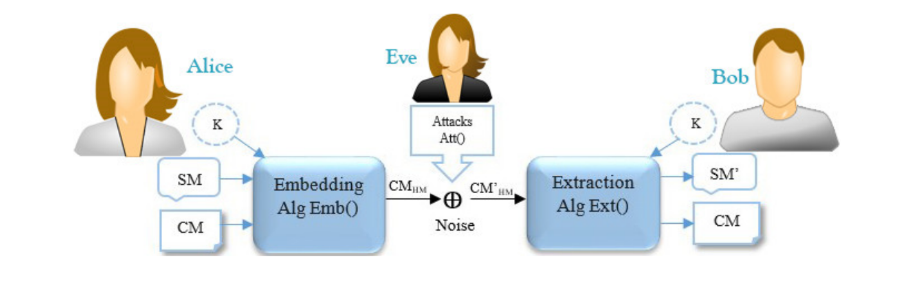
\includegraphics[scale=0.45]{modern_text_hiding.png}
\end{figure}

The proposed image intuitively explains the logic of the schema.
Alice who whishes to send a Secret Message(SM) to Bob, will produce a Cover
Message(CM), \emph{i.e.} an innocent message which will work as a carrier.
She will then embedd the SM into the CM using a steganographic algorithm
and, optionnally\footnote{This is the domain of cryptography}, securing it
with a key(K).
In the end she will pass the message to Eve, who will analyse it before
giving it to Bob.
Eve, an active warden, will use steganalysis tools in order to break the
cover taylored by Alice and will possibly distort the message in order to
make it unreadable to Bob.
Once the message arrives to Bob, he will apply the inverse steganographic
algorithm in order to read the message.
Since the message could be courrupted Bob will have to perform some error
correction in order to make the message readable again(whenever this is
possible).
To summarize the principal charachteristics of the message sent by Alice
are:
\begin{itemize}
    \item \emph{invisibility}: the message should not be noted by Eve
    \item \emph{capacity}: the CM must be large enough to embedd all the SM
    \item \emph{distortion roboustness}: the SM should resist the noise
        produced by Eve in the channel
\end{itemize}

\subsection{Steganography in text}
Now let us abandon the prison world to move to the digital domain.
We now want to propose intuitively some algorithm which could be exploited
to cover hidden messages into text.
The field of hidden-text encoding owes its growth to two main factors: the
introduction of the Unicode Standard and the growth in popularity of social
media and messenger applications.
The number of "invisible" characters introduced by the Unicode
standardization can be exploited by steganographic algorithms just as
invisible ink was exploited in handwritten steganography.
Combining this result with the fact that the modern society produces every
year more data than ever before in human history, the possibilities and the
threats brought by steganography in the digital world are basically
limitless.

\begin{figure}[h]
    \centering
    \caption{Text Hiding techniques}
    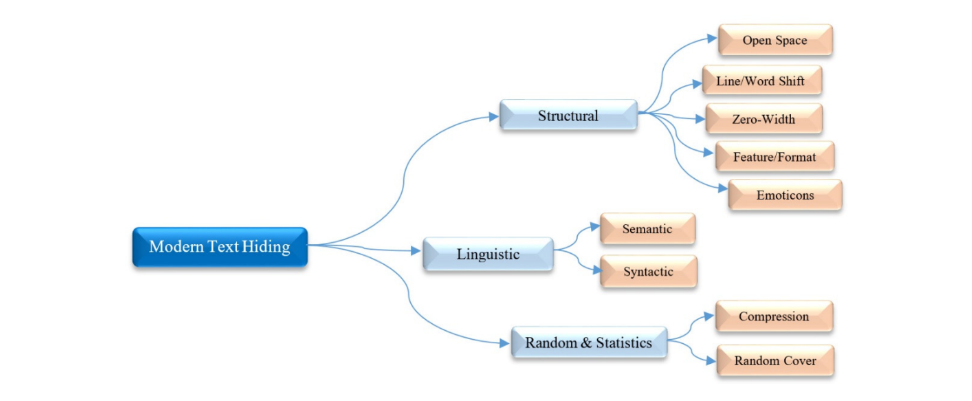
\includegraphics[scale=0.45]{text_hiding.png}
\end{figure}

As you can see the field is vast even here and unfortunately we will only
treat the most interesting points of the numerous ramifications.

\subsubsection{Structural}
This set of techniques consist in altering the structure of the document
rather than actively modifying the file. The case of \emph{open space} is
significant: the spaces are substituted by other invisible Unicode
character.
This technique is easily noticeable(even by the human eye) and not so much
rubust.
Similar is the \emph{zero width} techniques which exploits the zero width
characters present in the Unicode standard.
Even more visible are the format, color and alignement alterations of
\emph{Format}.
Much more interesting is the case of \emph{Emoticons} which has found secure
ground in the last period and which consist of assigning to each emojy a
code(letter or word).

\subsubsection{Linguistic}
Much more stable are the algorithms which exploits linguistic
characteristics in order to hide the presence of hidden bits.
In the \emph{Semantic} case the message is hidden inside abbreviations or
achronyms.
This method provides much more reliability and lower embedding capability
than the previous one.
Much worse and visible is the \emph{Syntactic} approach which consists in
changing symbols with others to represent some code.

\subsubsection{Random and Statistic}
These method start only from the SM and try to generate a CM.
They are usually much more time and resources consuming.
The \emph{Compression} method consists in compressing the text of the SM
using well known compression algorithms such as \emph{Huffman Coding}.
The so compressed text is then reordered to mimic the user-typed format or
at least a plausible one.
Not much more efficient is the \emph{Random Cover} approach where an
algorithm(\emph{AH4s}) is used to generate a long(and usually meaninglsess)
text from the specified SM.
The latter method is indeed very visible and also computationally expensive.

\subsection{steganalysis}

\subsubsection{Visual steganalysis}
This is a human powered technique which simply consists in reading the texts
searching for anomalies in the syntax, impagination and type of characters
used.
This type of analysis can only be performed by trained users and in most of
the scenarios simply detects the presence of hidden messagges without
retreiving it.
A common type of attack which could be performed by the user consciously(not
necessarily) is manually changing the structure of the message.
This may lead to the loss or irretrievability of the SM.

\subsubsection{Statistical steganalysis}
We have already treated this in the previous section, but now we will focus
our attention on the particular case of text steganography.
Since we don't want to treat the topic from a too mathematical perspective,
we will try not to enter into the mathematical technicalities.
The basic principle beneath is the assumption that it is possible to
describe the message with a probability function.
Recalling some basic principles of probability, if
$ x_1, x_2, x_3 \dots x_n $ are independent, then
$ p(x_1, x_2, x_3, ... x_n) = p(x_1) p(x_2) \dots p(x_n)$. 
Instead when they are not then
$$ p(x_1, x_2, x_3, ... x_n) = p(x_1) p(x_2 | x_1) p(x_3 | x_1, x_2) \dots
p(x_n | x_1, x_2, \dots, x_{n-1}) $$
Starting by the assumption that written text follows a logic schema and thus
that words are interdependently related, then by computing the probability
function of the text and comparing it to the one of the
\emph{stego-message}(assumed to be perturbed by steganography) we can detect
the presence of steganography in the text. 
This tells us that in theory is possible to detect whether a sequence of
characters follows a specific pattern or not, and it is in theory also
possible to retrieve the message from such prediction.
In \cite{fast-steg-method} the experiment presented shows that it is
possible to use a neural network to recognize patterns into text messages
which are proper of \emph{stego-messages}.


\end{document}